\newpage
\section{Rummets indvirken}
I den forrige sektion blev det undersøgt hvordan højtalerens eget frekvensrespons så ud. I virkeligheden vil dette respons dog være påvirket af det rum det er placeret i og derfor blev højtaleren flyttet til et 'virkeligt rum' - nærmere bestemt et klasselokale på IHA. Ved hjælp af rummet indvirkning ønskes en nærmere klarlægning af betydning af basrefleksens placerings i forhold til højtalerens frekvenskarakteristik.

En af CLIO-Pockets andre funktioner er, at den er i stand til, at måle impulsresponset i et rum. Dette blev gjort ved, at indstille softwarens parametre som der stod beskrevet i manualen,indstille til en såkaldt 'one-shot'-måling og herefter lave et 'klap' foran CLIO-mikrofonen. Resultatet af dette kan ses nedenfor - målt i både Pascal og dB Sound Pressure Level (SPL).
\begin{figure}[H]
	\centering
	\vspace{-12pt}
	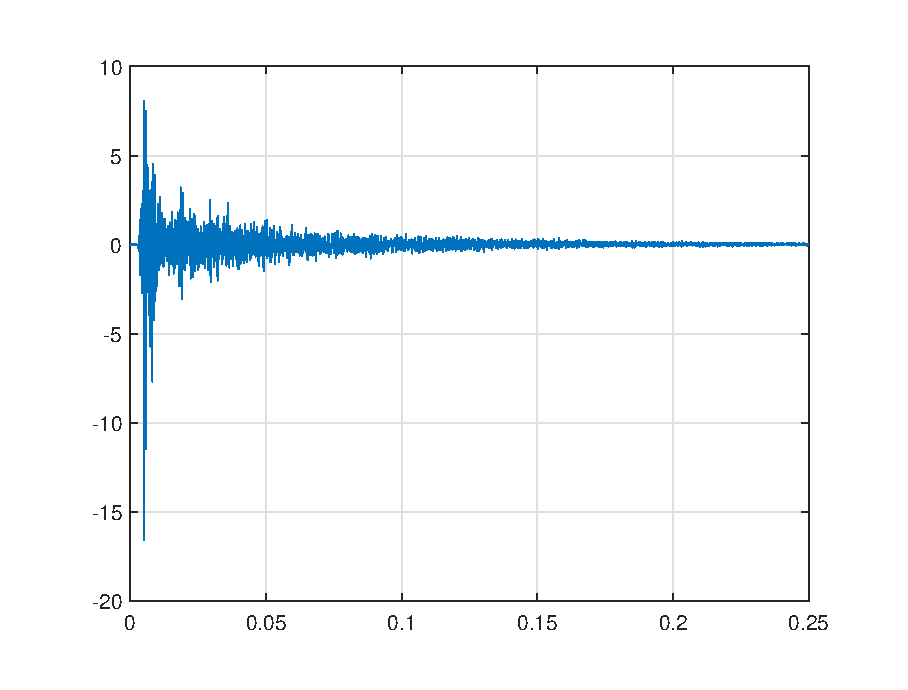
\includegraphics[width=\textwidth]{Billeder/Grafer/ImpulsResponse}
	\caption{Rummets impulsrespons i tidsdomænet}
\end{figure}

Ud fra denne ovenstående graf kan efterklangstiden $t_{60}$ i rummet også måles som den tid der skal gå, inden responset er faldet med \SI{60}{\decibel}. Denne blev målt til nær \SI{45}{\milli\second},som afviger en smule fra den analytisk beregnede efterklangstid i afsnit \ref{chapt:Sim}.

\newpage
Højtaleren blev placeret i et rum og med membranen placeret \SI{20}{\centi\meter} over gulvet og CLIO-mikrofonen i en afstand på \SI{1}{\meter} direkte foran membranen. Herefter blev der udført frekvenskarakteristik-målinger som i forrige afsnit. Resultatet af disse målinger - samt de simulerede målinger - kan ses nedenfor:
\begin{figure}[H]
	\centering
	\vspace{-12pt}
	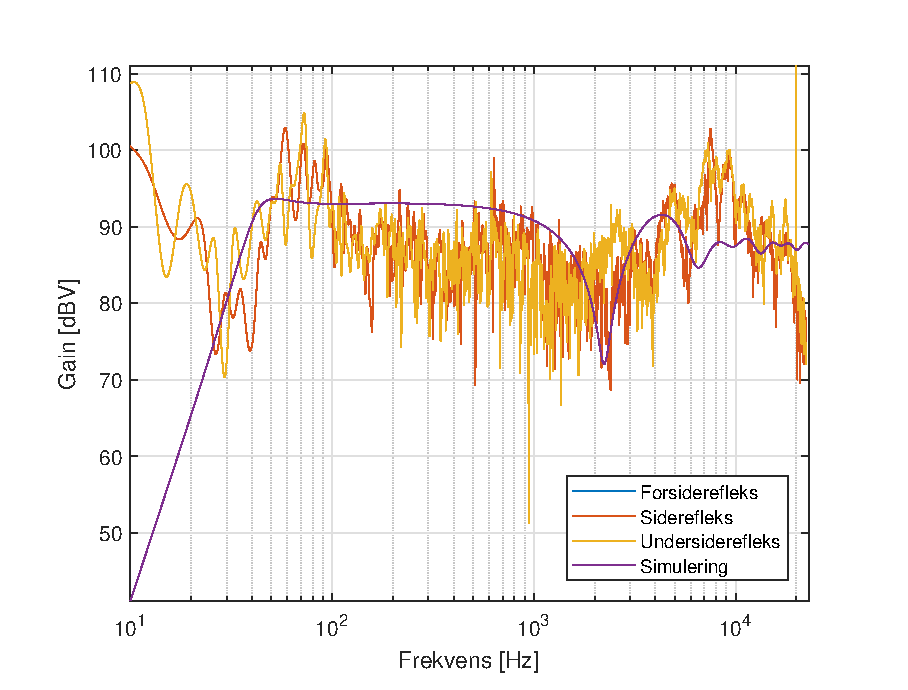
\includegraphics[width=\textwidth]{Billeder/Grafer/RealDirect}
	\caption{Basrefleksens betydning for frekvenskarakteristik (målt direkte)}
\end{figure}

Der er ikke umiddelbart muligt, at se nogen stor forskel i frekvenskarakteristikkerne da de ligger meget oven i hinanden. Det ses dog, at de simulerede data stemmer ret godt overens med de reelle måledata.

\newpage
På samme måde som før, blev højtaleren placeret i et rum med membranen placeret \SI{20}{\centi\meter} over gulvet. Denne gang blev CLIO-mikrofonen dog placeret i en højde på \SI{1,5}{\meter} over gulvet for at simulere en lytter. Resultatet af dette - samt de simulerede målinger - kan ses på grafen nedenfor:
\begin{figure}[H]
	\centering
	\vspace{-12pt}
	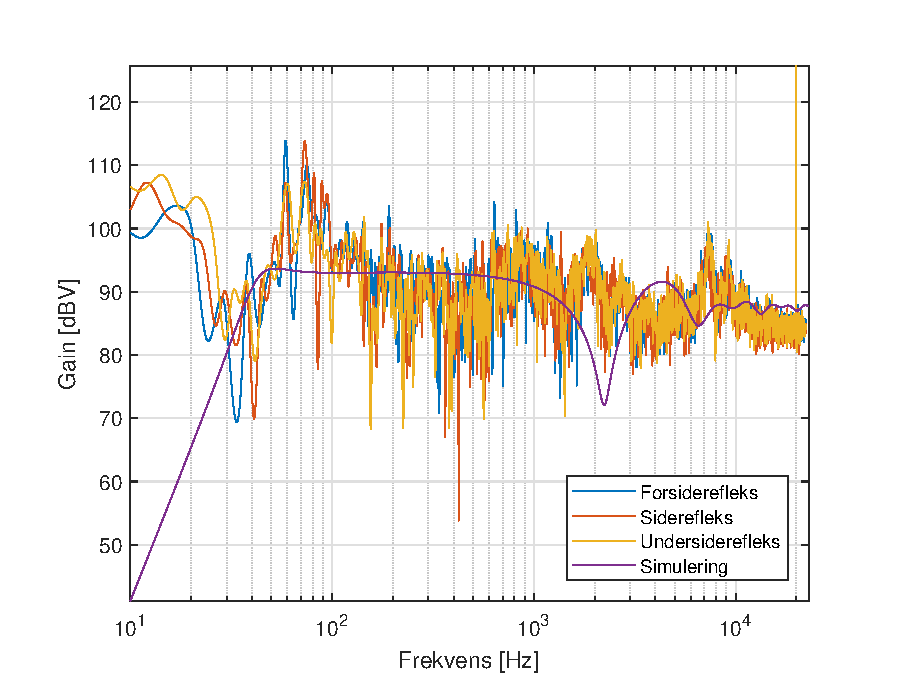
\includegraphics[width=\textwidth]{Billeder/Grafer/RealListen}
	\caption{Basrefleksens betydning for frekvenskarakteristik (målt i lyttehøjde)}
\end{figure}

Ligesom før kan det være svært at se forskel på de forskellige frekvenskarakteristikker, men det virker dog til, at undersiderefleksen har en smule højere forstærkning ved de lave frekvenser end de andre to placeringer.
\begin{figure}[H]
	\centering
	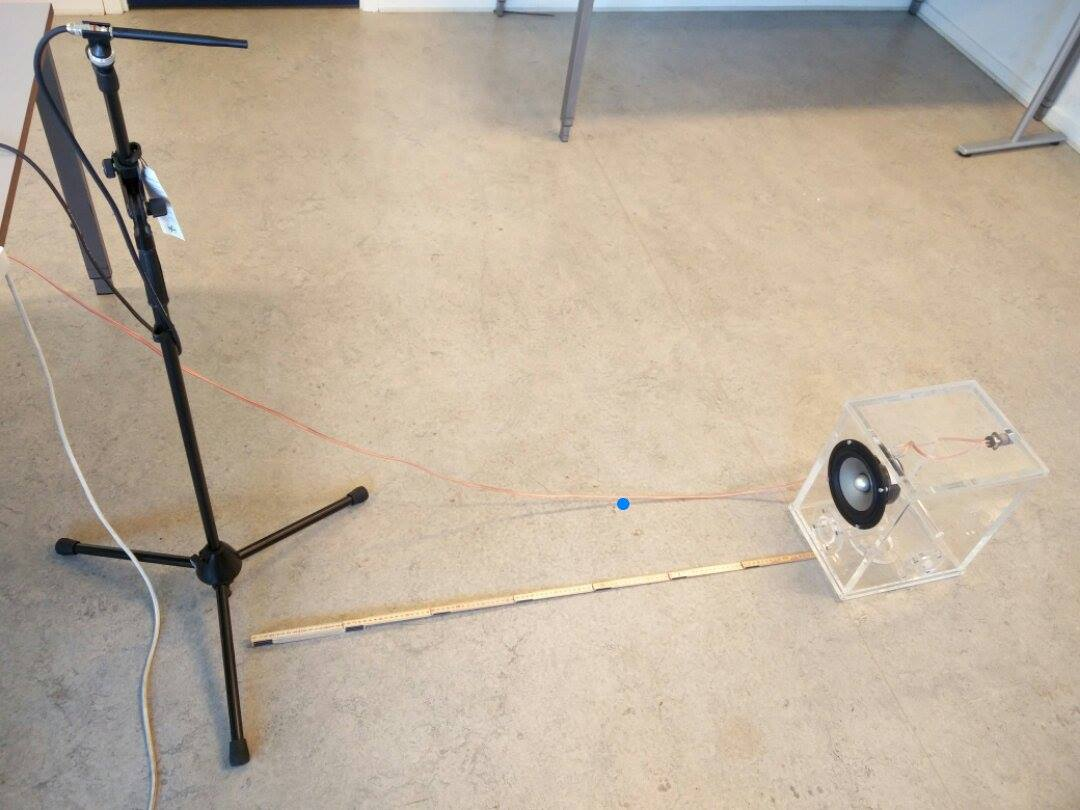
\includegraphics[width=0.5\textwidth]{Billeder/RealMaaling}
	\caption{Måleopstilling for rummets indvirken}
\end{figure}